
\section{Protokol WebRTC}\label{webRTC}

Tato část práce vychází převážně z knihy
\href{https://webrtcforthecurious.com/}{WebRTC For The Curious: Go beyond the
	APIs} \cite{WebRTCForTheCurious}.

\textit{Web Real-Time Communication} (\textit{WebRTC}) je protokol, který
umožňuje vytvoření bezpečného obousměrného \textit{peer-to-peer}
(\textit{P2P})\footnote{Peer-to-peer spojení dvou počítačů je takové spojení,
kde k výměně dat není třeba žádný server \cite{MerriamWebster-PeerToPeer}.}
spojení mezi dvěma klienty pro přeposílání audia, videa a libovolných dat v
reálném čase. Toto spojení je \textit{end-to-end šifrováno}
(E2EE)\footnote{End-to-end šifrování je metoda, kde třetí strany nemůžou číst
data, neboť klíče mají jen koncové strany. Příkladem je mnoho aplikací pro chat,
kde server nemůže číst zprávy uživatelů, neboť klíče mají jen klienti daných
uživatelé \cite{IBM-EndToEndEncryption}.}, což zaručuje, že žádná třetí strana
nemůže přeposílána data rozšifrovat \cite{WebRTCForTheCurious}.

WebRTC spojení je složeno ze \textit{stop} (\textit{tracks}) a datových kanálů
(\textit{data channels}). Stopa může být např. audio z mikrofonu či video z
kamery \cite{MDN-WebRTC-MediaStreamTrack}, tyto stopy mohou být přiřazeny do
tzv. \textit{streamů} (stream je často složen ze dvou stop -- audio a videa
např. z mikrofonu a kamery či z počítače
uživatele)~\cite{MDN-WebRTC-MediaStream}. Datové kanály se pak používají k
přenosu libovolných dat \cite{WebRTCORG-GettingStarted-DataChannels}.

\textit{Application Programming Interface} (\textit{API}) protokolu WebRTC je
specifikováno jen v~JavaScriptu, ale existují i jiné implementace
\cite{WebRTCForTheCurious}, jako je např. \href{pion/webrtc: Pure Go
	implementation of the WebRTC API}{Pion} \cite{GitHub-Pion-WebRTC} či
\href{https://github.com/webrtc-rs/webrtc}{WebRTC.rs}
\cite{GitHub-WebRTCRS-WebRTC}.

Protokol WebRTC se skládá z mnoha komponentů a využívá ke svému fungování mnoha
jiných protokolů \cite{WebRTCForTheCurious}. V této části si jednotlivé
komponenty rozebereme a popíšeme k čemu slouží.

\subsection{Spojování}\label{connecting}

Tradiční aplikace často používají model klient-server, kde má server fixovanou
známou IP adresu, kterou může klient využít pro komunikaci. Ve WebRTC tomu ale
tak není, neboť protokol je P2P, oba klienti jsou tedy zodpovědní za vytvoření
obousměrného spojení, což může být složité, ale má to své vyhody jako menší
zpoždění a E2EE, vývojář se zároveň nemusí starat o žádné servery
\cite{WebRTCForTheCurious}.

Pro vytvoření spojení se používá protokolu \textit{Interactive Connectivity
Establishment} (\textit{ICE}). Protokol ICE slouží k nalezení nejlepšího
způsobu, jak vytvořit spojení mezi dvěma klienty. Každý klient zveřejní své tzv.
\textit{ICE kandidáty}, což jsou v podstatě IP adresy a porty, na kterých je
klient dostižitelný (více v části \ref{ice})~\cite{WebRTCForTheCurious}. V této
části se zabýváme jen samotným výběrem těchto kandidátů, o tom, jak si klienti
předají informace o tom kandidátech se dozvíte v sekci \ref{signalling}.

\subsubsection{NAT}\label{nat}

\begin{figure}[H]
	\centering
	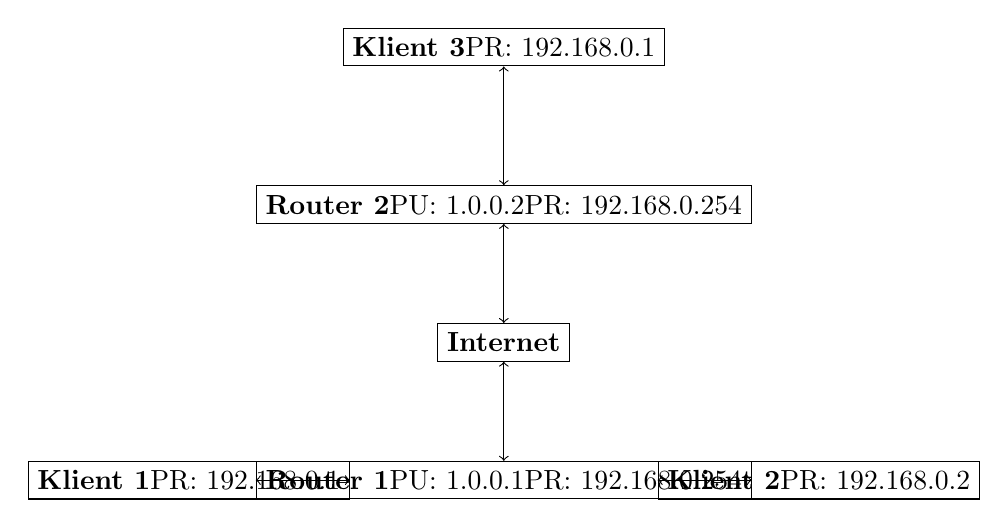
\begin{tikzpicture}
		\node[draw] (client3) at (0,3.75) {\textbf{Klient 3}\\PR: 192.168.0.1};
		\node[draw] (router2) at (0,1.75) {
			\textbf{Router 2}\\
			PU: 1.0.0.2\\
			PR: 192.168.0.254
		};
		
		\node[draw] (internet) at (0,0) {\textbf{Internet}};
		
		\node[draw] (router1) at (0,-1.75) {
			\textbf{Router 1}\\
			PU: 1.0.0.1\\
			PR: 192.168.0.254
		};
		\node[draw] (client1) at (-4,-1.75) {\textbf{Klient 1}\\PR: 192.168.0.1};
		\node[draw] (client2) at (4,-1.75) {\textbf{Klient 2}\\PR: 192.168.0.2};

		\draw[<->] (client1) -- (router1);
		\draw[<->] (client2) -- (router1);
		\draw[<->] (router1) -- (internet);

		\draw[<->] (internet) -- (router2);
		\draw[<->] (router2) -- (client3);
	\end{tikzpicture}
	\caption{NAT (\publicPrivateIP)}
	\label{natFig}
\end{figure}

Na obrázku \ref{natFig} můžeme vidět situaci, ve které by bylo snadné pro
klienta 1 poslat paket klientovi 2, neboť jsou na stejné síti. Ale pokud by
klient 3 chtěl poslat paket klientovi za routerem 2, situace by už byla
složitější, neboť klienti jsou na jiných sítích a je nutné využít veřejných IP
adres routerů, které ale klienti nutně neznají, zároveň je nutné, aby router
věděl, na jaký z klientů paket přeposlat \cite{WebRTCForTheCurious}.

Routery využívají k řešení této situace metodu \textit{Network Address
Translation} (\textit{NAT}). NAT umožňuje vytvořit mapování mezi IP adresou a
portem, které jsou viditelné zvenčí, a IP adresou a portem, které jsou viditelné v síti routeru \cite{WebRTCForTheCurious}.

Jednou z možností mapování je \textit{port forwarding}, jde o statické
namapování předem definovaného portu použitelného zvenčí sítě routeru na IP
adresu a port v siti routeru. Na obrázku \ref{natFig} by mohl router 2 mít
vytvořené takové mapování, že v případě, že zvenčí sítě přijde paket na port
\mintinline{text}{80}, router ho přesměruje na klienta 3 na port
\mintinline{text}{90}. Zároveň pošle-li klient 3 paket na router na port
\mintinline{text}{90}, bude přeposlán routerem přes port \mintinline{text}{80}.
Toto mapování je vhodné pro případy, kdy chceme, aby dané zařízení za routerem
bylo dostižitelné na IP adrese routeru na pevně daném portu
\cite{G2-WhatIsPortForwarding}. (Pro zjednodušení předpokládáme, že IP adresa
routeru je statická.)

Mapování ale nemusí být pevné a může existovat jen dočasně. Pošle-li klient 1
paket na IP adresu routeru 2 na port \mintinline{text}{80}, vybere router 1 port
a přepošle paket z tohoto portu. Když následně klient 3 pošle paket na router 1
na portu, ze kterého přišel paket první, router 1 rozpozná dle portu, že má
paket přeposlat klientovi 1. Toto mapování může ale v budoucnosti
zaniknout\footnote{Jak dlouho je mapování funkční závisí na mnoha faktorech.
Např. pokud je použit protokol TCP, mapování se ruší explicitně.}. Tento typ
mapování je nejčastější pro běžná zařízení \cite{WebRTCForTheCurious}.

\subsubsection{STUN}

\begin{figure}[H]
	\centering
	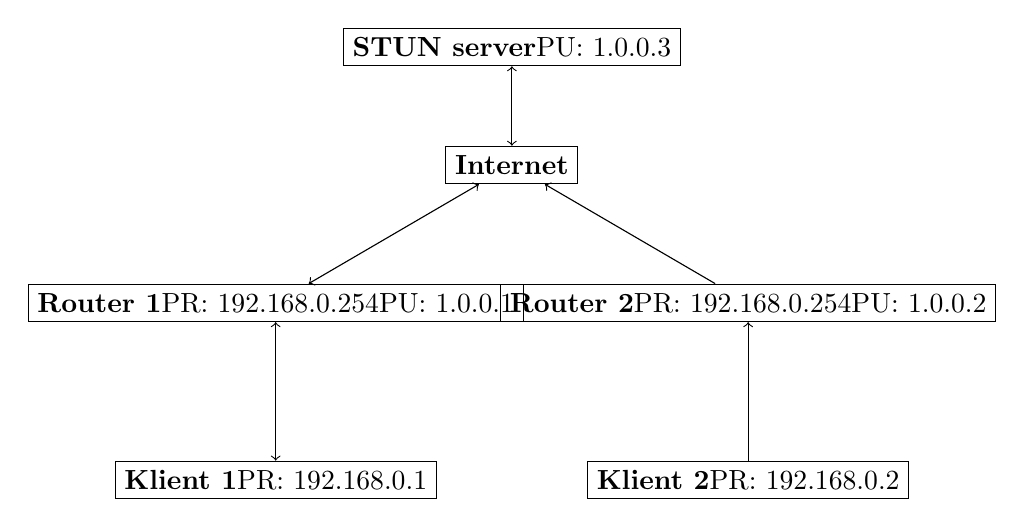
\begin{tikzpicture}
		\node[draw] (stunServer) at (0,1.5) {\textbf{STUN server}\\PU: 1.0.0.3};

		\node[draw] (internet) at (0,0) {\textbf{Internet}};

		\node[draw] (router1) at (-3,-1.75) {
			\textbf{Router 1}\\
			PR: 192.168.0.254\\
			PU: 1.0.0.1
		};
		\node[draw] (client2) at (3,-4) {\textbf{Klient 2}\\PR: 192.168.0.2};

		\node[draw] (router2) at (3,-1.75) {
			\textbf{Router 2}\\
			PR: 192.168.0.254\\
			PU: 1.0.0.2
		};
		\node[draw] (client1) at (-3,-4) {\textbf{Klient 1}\\PR: 192.168.0.1};

		\draw[<->] (client1) -- (router1);
		\draw[<->] (router1) -- (internet);
		\draw[<-] (internet) -- (router2);
		\draw[<-] (router2) -- (client2);

		\draw[<->] (internet) -- (stunServer);
	\end{tikzpicture}
	\caption{STUN (\publicPrivateIP)}
	\label{stun}
\end{figure}

\textit{Session Traversal Utilities for NAT} (\textit{STUN}) je protokol, který
umožňuje překonat problémy popsané v sekci \ref{nat}. Protokol
STUN byl vytvořen pro práci s \textit{NAT} (\textit{Network Address
Translation}) \cite{WebRTCForTheCurious}.

V síti, která je vidět na obrázku \ref{stun}, klient 1 pošle \textit{STUN
	Binding Request} STUN serveru, který má známou statickou veřejnou IP adresu.
Router 1 využije metody NAT pro vytvoření mapování na určitém portu. STUN
server pomocí \textit{STUN Binding Response} pošle na router 1 informace o
tom, z jaké IP adresy a portu request přišel. Protože bylo na routeru 1
vytvořeno mapování, ví, že pokud přijde zpráva na daném portu, má ji
přeposlat klientovi 1, ten poté ze STUN Binding Response může vyčíst, jaká
je jeho \textit{Mapped Address} (někdy také \textit{veřejná IP adresa} či
\textit{Server Reflexive Candidate}). V~podstatě se jedná o automatické
dynamické port forwardování~\cite{WebRTCForTheCurious}.

Bohužel Mapped Address vůbec nemusí být užitečná, pokud je použito NAT mapování
typu \textit{Address Dependent}, což znamená, že router 1 přijímá na daném
mapování pakety pouze od STUN serveru\footnote{Address Dependent mapování lze
často také nalézt pod pojmem \textit{Symmetric} NAT. Tento pojem je ale
nepřesný, neboť reálné NAT často nelze snadno klasifikovat do kategorií
\cite{IETF-RFC4787}.}. STUN naštěstí umožňuje zjištění typu NAT mapování, takže
klient předem ví, jestli ho bude možné kontaktovat \cite{WebRTCForTheCurious}.

\subsubsection{TURN}

\begin{figure}[H]
	\centering
	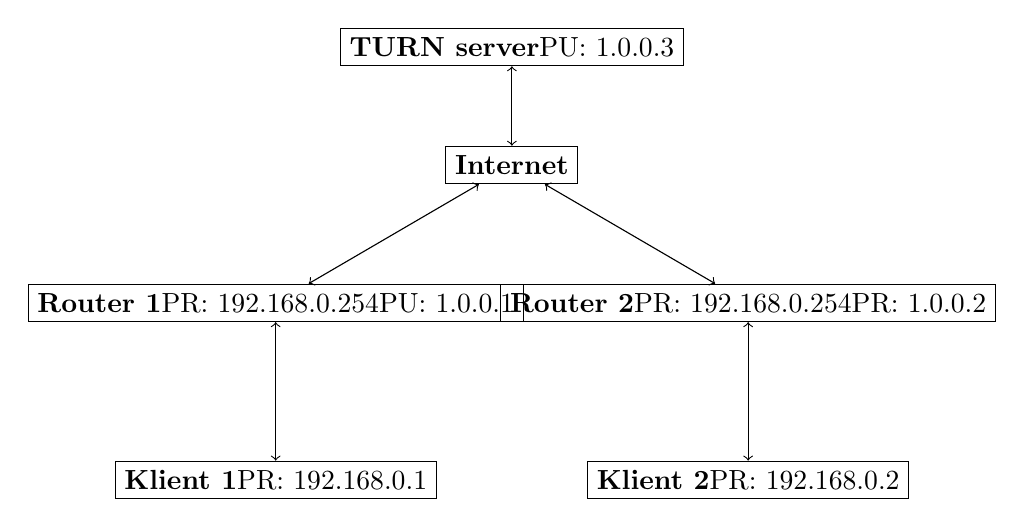
\begin{tikzpicture}
		\node[draw] (turnServer) at (0,1.5) {\textbf{TURN server}\\PU: 1.0.0.3};
		\node[draw] (internet) at (0,0) {\textbf{Internet}};

		\node[draw] (router1) at (-3,-1.75) {
			\textbf{Router 1}\\
			PR: 192.168.0.254\\
			PU: 1.0.0.1
		};
		\node[draw] (client1) at (-3,-4) {\textbf{Klient 1}\\PR: 192.168.0.1};

		\node[draw] (router2) at (3,-1.75) {
			\textbf{Router 2}\\
			PR: 192.168.0.254\\
			PR: 1.0.0.2
		};
		\node[draw] (client2) at (3,-4) {\textbf{Klient 2}\\PR: 192.168.0.2};

		\draw[<->] (client1) -- (router1);
		\draw[<->] (router1) -- (internet);
		\draw[<->] (turnServer) -- (internet);
		\draw[<->] (internet) -- (router2);
		\draw[<->] (router2) -- (client2);
	\end{tikzpicture}
	\caption{TURN (\publicPrivateIP)}
	\label{turn}
\end{figure}

\textit{Traversal Using Relays around NAT} (\textit{TURN}) je metoda, která
umožňuje vytvořit spojení i v případě, že je NAT mapování Address Dependent, či
pokud je klient za jinak restriktivním firewallem. TURN lze také využít,
přeje-li si klient, aby druhý klient neznal jeho IP adresu
\cite{WebRTCForTheCurious}.

Jak je vidět na obrázku \ref{turn}, TURN server funguje jako proxy (prostředník),
přes které jsou přeposílána data. Přeje-li si klient 1 využít TURN server, musí
nejdříve vytvořit tzv. \textit{alokaci}, která je následně využita k přeposílání
dat. Aby alokaci klient 1 vytvořil, musí serveru poskytnout uživatelské jméno,
heslo, protokol (může být UDP nebo TCP) a port~\cite{WebRTCForTheCurious}.

Podaří-li se alokaci vytvořit, odpověď TURN serveru obsahuje Mapped Address
(stejně jako v případě STUN), \textit{Lifetime}, což je doba, po kterou bude
alokace aktivní, \textit{Relayed Address}, což je adresa, kterou klient 1 předá
ostatním klientům. Pokud jsou na ni poslány pakety, budou TURN serverem
přesměrovány na klienta, který vytvořil danou alokaci
\cite{WebRTCForTheCurious}.

Nyní musí klient 2 poslat TURN serveru STUN Binding Request a klientovi 1 sdělit
svou Mapped Address. Klient 1 pak může klientovi 2 povolit, aby na danou alokaci
posílal pakety \cite{WebRTCForTheCurious}.

Klient 1 poté může poslat \textit{Send Indication}, která obsahuje data, které se
mají přeposlat klientovi 2 \cite{WebRTCForTheCurious}.

Posílá-li se velké množství paketů, může být nevýhodné, aby každý z nich
obsahoval IP adresu a port. Je tedy možné vytvořit tzv. \textit{kanál}
(\textit{Channel}), mající své \textit{ID kanálu} (\textit{Channel ID}). Klient
pak kanál používá v paketech místo IP adresy a portu. Paket je poté na TURN
serveru upraven a IP adresa a port dodány \cite{WebRTCForTheCurious}.

Vzhledem k tomu, že alokace jsou časově omezeny, klient může poslat
\textit{Refresh} request, který by měl prodloužit lifetime dané alokace
\cite{WebRTCForTheCurious}.

\subsubsection{ICE}\label{ice}

\textit{Interactive Connectivity Establishment} (\textit{ICE}) je protokol,
který najde všechny možné způsoby, jak spojit dva dané klienty, a následně jeden
z nich vybere \cite{WebRTCForTheCurious}.

Páry adres a portů, které je možné využít pro spojení dvou klientů, se nazývají
\textit{páry kandidátů}. Může se jednat o privátní adresy, veřejné adresy, či
Relayed Adresy. Klienti komunikují pomocí \textit{ICE ping paketů}
\cite{WebRTCForTheCurious}.

ICE klient je buď \textit{controlling}, nebo \textit{controlled} -- klient,
který je controlling, je ten, který vybere vhodný pár kandidátů; obvykle je
controlling klient ten, který zahájil spojování~\cite{WebRTCForTheCurious}.

Nabízí-li každá strana 2 kandidáty, existují pak 4 páry kandidátů. Klienti
využijí ICE ping pakety, aby ověřili, které páry jsou funkční. Ty páry, u
kterých došlo k výměně dat, jsou pak označeny za \textit{validní kandidáty}.
Controlling klient následně vybere jeden z validních párů a označí ho za
\textit{nominovaný pár}. Klienti se pak znovu pokusí o obousměrnou komunikaci
pomocí tohoto páru, a je-li úspěšná, stává se z daného párů \textit{vybraný pár
	kandidátů} \cite{WebRTCForTheCurious}.

Dojde-li po vytvoření spojení k potížím (např. vyprší NAT mapování nebo selže
TURN server), celý proces začne znovu \cite{WebRTCForTheCurious}.

\subsubsection{Způsobí přechod na IPv6 smrt ICE a STUN?}

NAT původně vzniklo jako způsob řešení nedostatku IPv4 adres, ale za léta svého
vývoje se jejich význam rozšířil, neboť zároveň poskytují jednu z vrstev
zabezpečení \cite{Quora-WillIPv6KillSTUNAndICE}.

Přestože postupný přechod na IPv6 je nevyhnutelný, je nepravděpodobné, že by
technologie jako NAT zmizely, a tak je smysluplné předpokládat, že technologie
jako ICE a STUN rovněž zůstanou relevantní \cite{Quora-WillIPv6KillSTUNAndICE}.

\subsection{Posílání médií}

WebRTC umožňuje posílat neomezené množství audio a video stop, které buď mohou
být nezávislé, nebo mohou být součástí streamu. Typickým příkladem je uživatel,
který v jednom streamu posílá audio stopu ze svého mikrofonu a video stopu ze
své kamery a v druhém streamu audio stopu a video stopu ze svého počítače.
Dalším příkladem je server, který přeposílá streamy jiných uživatelů, jak je
popsáno v části \ref{connectionModels} \cite{WebRTCForTheCurious}.

\subsubsection{RTP}\label{rtp}

\textit{Real-time Transport Protocol} (\textit{RTP}) je protokol, který se
využívá pro přenos médií. RTP umožňuje posílání několik streamů (ve WebRTC je
RTP stream jedna stopa) přes jedno peer-spojení. RTP zároveň dává vývojáři
informace o časování a pořadí paketů, je ale nezávislé na kodeku
\cite{WebRTCForTheCurious}.

\subsubsection{RTCP}\label{rtcp}

\textit{RTP Control Protocol} (\textit{RTCP}) je protokol, který umožňuje
přeposílání metadat o RTP spojení. Obvykle se jedná o metadata jako je např.
ztráta paketů \cite{WebRTCForTheCurious}.

\subsection{Posílání dat -- SCTP}\label{sctp}

\textit{Stream Control Transmission Protocol} (\textit{SCTP}) je protokol, který
umožňuje přeposílání libovolných dat pomocí WebRTC. WebRTC \textit{datové
	kanály} (\textit{data channels}) jsou jeho abstrakcí. Každé WebRTC spojení může
obsahovat neomezeně datových kanálů (podobně jako je to u RTP streamů)
\cite{WebRTCForTheCurious}.

\subsection{Šifrování}

Všechna data přeposílána v rámci WebRTC spojení jsou E2EE
\cite{WebRTCForTheCurious}, což je zajištěno pomocí dvou protokolů, které si
popíšeme níže.

\subsubsection{DTLS}

\textit{Datagram Transport Layer Security} (\textit{DTLS}) je protokol podobný
protokolu TLS, ale je určený pro šifrování dat, která jsou posílána přes
protokol UDP místo TCP \cite{WebRTCForTheCurious}.

\subsubsection{SRTP}\label{srtp}

\textit{Secure Real-time Transport Protocol} (\textit{SRTP}) je protokol, který
využívá externích klíčů vygenerovaných DTLS k šifrování RTP paketů
\cite{WebRTCForTheCurious}.

\subsection{Signalling}\label{signalling}

\begin{figure}[H]
	\centering
	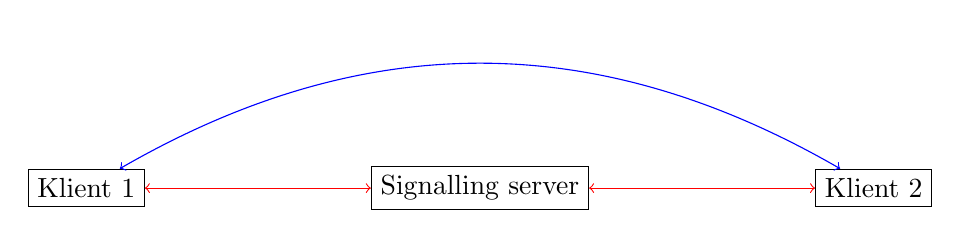
\begin{tikzpicture}
		\node[draw] (server) at (0,0) {Signalling server};
		\node[draw] (client1) at (-5, 0) {Klient 1};
		\node[draw] (client2) at (5, 0) {Klient 2};

		\draw[red, <->] (server) -- (client1);
		\draw[red, <->] (server) -- (client2);
		\draw[blue, <->] (client1) edge[bend left=30] (client2);
	\end{tikzpicture}
	\caption{Signalling}
	\label{signallingServer}
\end{figure}

\textit{Signalling} je zásadní součást WebRTC. Jedná se o proces při kterém si
klienti vyměňují pomocí tzv. \textit{signalling serveru} ICE kandidáty a
informace o tom, jaká média a data plánují posílat, jaké kodeky\footnote{Kodek
je hardware či software, který se využívá pro zakódování, či rozkódování médii
\cite{Britannica-Codec,TechTarget-Codec}.} podporují atp. Zprávy, které si
klienti pomocí signalling serveru vyměňují, se nazývají \textit{session
descriptions}, jsou ve formátu, který je definován protokolem zvaným
\textit{Session Description Protocol} (\textit{SDP}) (místo \textit{session
description} se někdy píše jen \textit{SDP}) \cite{WebRTCForTheCurious}.
Signalling server není nijak standardizován, jedinou podmínkou je výměna SDP,
což vede k tomu, že aplikace často nejsou mezi sebou kompatibilní
\cite{MDN-Web-SignalingAndVideoCalling}.

Chce-li klient 1 volat klienta 2, vygeneruje tzv. \textit{session description
offer} (\textit{SDP offer}), kterou pomocí signalling serveru přepošle klientovi
2. Chce-li klient 2 hovor přijmout, vygeneruje tzv. \textit{session description
answer} (\textit{SDP answer}), kterou naopak přepošle klientovi 1. Poté, co
dojde k výměně session descriptions, klienti budou nejspíše schopní vytvořit P2P
spojení. Tento proces se nazývá
\textit{negotiation}
\cite{WebRTCForTheCurious,MozillaBlog-PerfectNegotiation}.

Dojde-li během hovoru ke změnám spojení (změní se stopy, které klienti posílají,
či se změní pozice klienta na síti), proběhne tzv. \textit{renegotiation}, kdy
se proces výměny session descriptions opakuje
\cite{MozillaBlog-PerfectNegotiation}.

SDP se skládá z \textit{párů klíč-hodnota} (\textit{key-value pairs}). Každý pár
má formát \mintinline{text}{<klíč>=<hodnota>}. SDP může stejný klíč obsahovat
několikrát. Záleží na pořadí jednotlivých řádků -- SDP začíná obecnými
informacemi o spojení, které jsou následovány jednotlivými média-sekcemi, které
popisují obousměrného stopy \cite{WebRTCForTheCurious}. Je-li hodnota
nedefinovaná, používá se znak \mintinline{text}{-} \cite{IETF-RFC8866}. SDP
podporuje několik klíčů, WebRTC využívá následující
\cite{WebRTCForTheCurious,IETF-RFC8866}:

\begin{itemize}
	\item \mintinline{text}{v} -- značí verzi, která je vždy \mintinline{text}{0}
	\item \mintinline{text}{o} -- popisuje tvůrce spojení, slouží jako jeho
	      unikátní identifikátor, skládá se z:
	      \begin{itemize}
		      \item \mintinline{text}{username} -- ID uživatele, který zahájil spojení
		      \item \mintinline{text}{sess-id} -- unikátní číslo, které
		            identifikuje spojení
		      \item \mintinline{text}{sess-version} -- verze session
		            description, která by se měla po každé změně zvýšit
		      \item \mintinline{text}{nettype} -- typ sítě, je vždy
		            \mintinline{text}{IN} (internet)
		      \item \mintinline{text}{addrtype} -- typ adresy, je buď
		            \mintinline{text}{IP4}, nebo \mintinline{text}{IP6}
		      \item \mintinline{text}{unicast-address} -- IP adresa tvůrce spojení
	      \end{itemize}
	\item \mintinline{text}{s} -- název session, SDP nesmí obsahovat více než
	      jeden klíč \mintinline{text}{s}
	\item \mintinline{text}{c} -- informace o spojení, pro WebRTC není klíč
	      \mintinline{text}{c} příliš zásadní, neboť se pro spojování využívá
	      protokolu ICE (více v části \ref{connecting}), skládá se z:
	      \begin{itemize}
		      \item \mintinline{text}{nettype} -- typ sítě, je vždy
		            \mintinline{text}{IN} (internet)
		      \item \mintinline{text}{addrtype} -- typ adresy, je buď
		            \mintinline{text}{IP4}, nebo \mintinline{text}{IP6}
		      \item \mintinline{text}{connection-address} -- IP adresa využita
		            ke spojení
	      \end{itemize}
	\item klíč \mintinline{text}{t} -- čas, kdy spojení začíná a končí, skládá
	      se z:
	      \begin{itemize}
		      \item \mintinline{text}{start-time} -- čas, kdy spojení začne; pokud je
		            \mintinline{text}{0}, spojení je permanentní
		      \item \mintinline{text}{stop-time} -- čas, kdy spojení skončí; pokud je
		            \mintinline{text}{0}, doba spojení není omezena
	      \end{itemize}
	\item \mintinline{text}{a} -- atribut, jeho formát je
	      \mintinline{text}{a=<jméno>:<hodnota>}; SDP může obsahovat několik
	      klíčů \mintinline{text}{a}, ať už pro celé spojení, nebo pro
	      specifickou média-sekci
	\item \mintinline{text}{m} -- popis médií, skládá se z:
	      \begin{itemize}
		      \item \mintinline{text}{media} -- typ média, je buď
		            \mintinline{text}{audio}, \mintinline{text}{video},
		            \mintinline{text}{application}, \mintinline{text}{text},
		            nebo \mintinline{text}{message}
		      \item \mintinline{text}{port} -- port, který je využit k posílání
		            dat
		      \item \mintinline{text}{proto} -- protokol, hodnoty mohou být:
		            \begin{itemize}
			            \item \mintinline{text}{udp} -- data jsou posílána přímo
			                  přes protokol UDP
			            \item \mintinline{text}{RTP/AVP} -- data jsou posílána
			                  pomocí protokolu RTP (více v části \ref{rtp}) s
			                  profilem pro audio a video
			            \item \mintinline{text}{RTP/SAVP} -- data jsou posílána
			                  pomocí protokolu SRTP (více v části \ref{srtp})
			            \item \mintinline{text}{RTP/SAVPF} -- data jsou posílána
			                  pomocí protokolu SRTP s podporou pro RTCP (více v
			                  části \ref{rtcp})
		            \end{itemize}
		      \item \mintinline{text}{fmt} -- seznam čísel, která určují
		            podporované formáty dat; čísla od \mintinline{text}{0} do
		            \mintinline{text}{95} referují ke specifickým formátům; u
		            čísel od \mintinline{text}{96} do \mintinline{text}{127} se
		            využívá \mintinline{text}{a=rtpmap:<fmt> <codec>} pro
		            specifikaci kodeku
	      \end{itemize}
\end{itemize}

SDP podporuje několik různých atributů, ty následující jsou zásadní pro funování
WebRTC \cite{WebRTCForTheCurious,IETF-RFC8866,IETF-RFC5888,IETF-RFC8841}:
\begin{itemize}
	\item \mintinline{text}{a=group:BUNDLE} značí, že přes jedno peer spojení
	      posíláme více stop; některé implementace vytváří jedno peer spojení na
	      každou stopu, což ale není doporučeno
	\item \mintinline{text}{a=sendrecv}, \mintinline{text}{a=sendonly},
	      \mintinline{text}{a=recvonly} a \mintinline{text}{a=inactive} --
	      značí, směr dat dané média sekce; oba klienti by se měli shodnout na
	      směru dat, obsahuje-li tedy SDP offer \mintinline{text}{a=sendonly},
	      SDP answer by měla obsahovat \mintinline{text}{a=recvonly} pro danou
	      média-sekci
	\item \mintinline{text}{a=mid} -- číslo média-sekce
	\item \mintinline{text}{a=msid} -- ID stopy a streamu, má formát
	      \mintinline{text}{<ID streamu> <ID stopy>}
	\item \mintinline{text}{a=rtpmap} -- zmíněno v předchozím odstavci
	\item \mintinline{text}{a=sctp-port} -- port používaný protokolem SCTP (více
	      v části \ref{sctp})
	\item \mintinline{text}{a=max-message-size} -- maximální velikost zprávy v
	      bytech
\end{itemize}

SDP zároveň podporuje několik atributů, které se využívají pro nastavení ICE a
výměnu ICE kandidátů \cite{WebRTCForTheCurious,IETF-RFC8839}:
\begin{itemize}
	\item \mintinline{text}{a=ice-ufrag} -- uživatelské jméno, používáno pro
	ověření integrity
	\item \mintinline{text}{a=ice-pwd} -- heslo, používáno pro ověření integrity
	\item \mintinline{text}{a=ice-options} -- specifikuje rozšíření, které
	klient podporuje
	\item \mintinline{text}{a=candidate} -- je na úrovni média-sekce a
	specifikuje informace o daném ICE kandidátu
\end{itemize}

\begin{minted}[breaklines,fontsize=\footnotesize]{text}
v=0
o=- 2021867665009852994 2 IN IP4 127.0.0.1
s=-
c=IN IP4 192.168.1.1
t=0 0
a=group:BUNDLE 0 1
a=ice-ufrag:o6S/
a=ice-pwd:mXxyUi9PVAiuCPvl
a=ice-options:trickle
m=audio 4000 RTP/AVP 0 111
a=mid:0
a=sendrecv
a=candidate:foundation 1 udp 2130706431 192.168.1.1 53165 typ host generation 0
a=end-of-candidates
a=msid:yvKPspsHcYcwGFTw DfQnKjQQuweLFdV
a=rtpmap:111 OPUS/48000/2
m=video 4000 RTP/AVP 96
a=mid:1
a=sendonly
a=msid:yvKPspsHcYcwGFTw Ii65zvjKITaFf0T
a=rtpmap:96 VP8/90000
m=application 9 UDP/DTLS/SCTP webrtc-datachannel
a=mid:2
a=sctp-port:5000
a=max-message-size:262144
\end{minted}

Výše můžeme vidět příklad reálného SDP, které obsahuje 3 média-sekce. Obě
používají port \mintinline{text}{4000} a protokol \mintinline{text}{RTP/AVP}. V
klíči \mintinline{text}{o} je důležité třetí pole s hodnotou
\mintinline{text}{2}, která indikuje verzi session description. Klíč
\mintinline{text}{s} nemá hodnotu, spojení je tedy bez názvu. Klíč
\mintinline{text}{c} je pak pro WebRTC nepodstatný.

První sekce je \mintinline{text}{audio}, její \mintinline{text}{mid} je
\mintinline{text}{0} a její směr je \mintinline{text}{sendrecv}, takže umožňuje
přijímání i posílání audio stopy Formát je dynamický a z
\mintinline{text}{a=rtpmap} lze vidět, že \mintinline{text}{111} značí, že se
jedná o kodek Opus. Můžeme si rovněž povšimnout specifikace ID streamu a stopy.

Druhá sekce je \mintinline{text}{video}, její \mintinline{text}{mid} je
\mintinline{text}{1} a její směr je \mintinline{text}{sendonly}, klient je tedy
ochotný používat tuto média-sekci pro posílání videa. Formát je opět dynamický,
z \mintinline{text}{a=rtpmap} lze vidět, že číslo \mintinline{text}{96} značí,
že se jedná o kodek VP8. Je také vidět, že stopa patří do stejného streamu jako
stopa v první media sekci.

Třetí sekce je \mintinline{text}{application} a popisuje datový kanál. Její
\mintinline{text}{mid} je \mintinline{text}{2}. Protokol SCTP využívá port
\mintinline{text}{5000} a maximální velikost zprávy je \mintinline{text}{262144}
\si{\byte}, což je \mintinline{text}{256} \si{\kibi\byte}.

Další klíče se týkají protokolu ICE, který je popsán v části \ref{ice}.
